%%%%%%%%%%%%%%%%%%%%%%%%%%%%%%%%%%%%%%%%%
% Wenneker Assignment
% LaTeX Template +
% Structure Specification File
% Version 2.0 (12/1/2019)
%
% This template originates from:
% http://www.LaTeXTemplates.com
%
% Authors:
% Vel (vel@LaTeXTemplates.com)
% Frits Wenneker
%
% License:
% CC BY-NC-SA 3.0 (http://creativecommons.org/licenses/by-nc-sa/3.0/)
% 
%%%%%%%%%%%%%%%%%%%%%%%%%%%%%%%%%%%%%%%%%

\documentclass[11pt]{scrartcl} % Font size

% Package declarations
\usepackage{algorithm2e}
\usepackage{amsmath, amsfonts, amsthm} % Math packages
\usepackage{listings} % Code listings, with syntax highlighting
\usepackage{amsthm}
\usepackage{todonotes}
\usepackage[english]{babel} % English language hyphenation
\usepackage{graphicx} % Required for inserting images
\usepackage{booktabs} % Required for better horizontal rules in tables
\usepackage{enumitem} % Required for list customisation
\usepackage{geometry} % Required for adjusting page dimensions and margins
\usepackage[utf8]{inputenc} % Required for inputting international characters
\usepackage[T1]{fontenc} % Use 8-bit encoding
\usepackage{fourier} % Use the Adobe Utopia font for the document
\usepackage{sectsty} % Allows customising section commands
\usepackage{scrlayer-scrpage} % Required for customising headers and footers
\usepackage[a-1b]{pdfx}
\usepackage[pdfa]{hyperref}
\usepackage{url}
\usepackage{soul}
\usepackage{titlesec}
\usepackage{xcolor}
\usepackage[capitalise]{cleveref}
\usepackage{fancyvrb}
\usepackage{javahighlight}

\theoremstyle{plain}

%\newtheorem*{theorem*}{Theorem}
%\newtheorem{theorem}{Theorem}

%\newtheorem*{definition*}{Definition}
%\newtheorem{definition}{Definition}

%\graphicspath{{Figures/}{./}} % Specifies where to look for included images (trailing slash required)

%\numberwithin{equation}{section} % Number equations within sections (i.e. 1.1, 1.2, 2.1, 2.2 instead of 1, 2, 3, 4)
%\numberwithin{figure}{section} % Number figures within sections (i.e. 1.1, 1.2, 2.1, 2.2 instead of 1, 2, 3, 4)
%\numberwithin{table}{section} % Number tables within sections (i.e. 1.1, 1.2, 2.1, 2.2 instead of 1, 2, 3, 4)

\setlength\parindent{0pt} % Removes all indentation from paragraphs

\setlist{noitemsep} % No spacing between list items

\geometry{
	paper=a4paper, % Paper size
	top=2.5cm, % Top margin
	bottom=2.5cm,%3cm, % Bottom margin
	left=2cm,%3cm, % Left margin
	right=2cm,%3cm, % Right margin
	headheight=0.75cm, % Header height
	footskip=1.5cm, % Space from the bottom margin to the baseline of the footer
	headsep=0.75cm, % Space from the top margin to the baseline of the header
	%showframe, % Uncomment to show how the type block is set on the page
}

\sectionfont{\vspace{6pt}\centering\normalfont\scshape} % \section{} styling
\subsectionfont{\normalfont\bfseries} % \subsection{} styling
\subsubsectionfont{\normalfont\itshape} % \subsubsection{} styling
\paragraphfont{\normalfont\scshape} % \paragraph{} styling

%\ohead*{} % Right header
%\ihead*{} % Left header
%\chead*{} % Centre header

%\ofoot*{} % Right footer
%\ifoot*{} % Left footer
%\cfoot*{\pagemark} % Centre footer

%% This declares a command \Comment
%% The argument will be surrounded by /* ... */
%% Used for pseudocode
\SetKwComment{Comment}{/* }{ */}
%% For adding 'function-like captions' as algorithms captions
\RestyleAlgo{ruled}


\title{	
	\normalfont\normalsize
	\textsc{University of Trento}\\ %
	\vspace{6pt}%
	\rule{\linewidth}{0.5pt}%
	\vspace{15pt} %
	{\huge Raft Simulator Evaluation}\\ % yeah, we could find a better title
	\vspace{6pt}%
	\rule{\linewidth}{2pt}\\
	\vspace{6pt}
}

\author{\LARGE Paolo Chistè, Matteo Franzil, Andrea Stedile}

\date{\normalsize\today}

\begin{document}

\maketitle % Print the title

\begin{abstract}

\centering
\bfseries%
\textsc{Abstract.} 
\vspace{1em}

Raft is a distributed consensus algorithm for managing a replicated log.
It is an efficient, understandable algorithm that is easier to implement than protocols such as Paxos, and offers equivalent performance and guarantees.
In this paper, we describe the implementation of a simulator of Raft using the Java language and Akka actor toolkit.
Our simulator comprises a Graphical User Interface, which provides a real-time view of the state of the servers in the cluster, allows the user to crash and resume the servers and submit new commands to be replicated.
% Our results show that the Raft protocol behaved correctly under the paper's assumption, while resulting scalable and easy to manage with the provided GUI.
% Andrea: Questa cosa sopra è ovvia; dato che il protocollo è formalmente verificato allora non vi è dubbio che funzioni
% TODO:
% The strength of the simulator is to enable the user to learn and appreciate the Raft protocol...

\end{abstract}

\section{Introduction}
%{\huge Da riscrivere probabilmente}
The \textbf{distributed consensus problem} is an unsolvable problem in Computer Science. Even with the most benign of assumptions, it is possible to prove that any algorithm that tries to solve the problem can enter in an inconsistent state by simply delaying the delivery of a message. \cite{fischer_impossibility_nodate}.

However, this theoretically impossible problem is solvable ``in practice'', by relaxation of one or more of its requirements. Paxos \cite{lamport_part-time_1998} is one of the first of these algorithms. Many modern implementations are based on Paxos, but with major modifications to its initial description. This is in part motivated by the intrinsic complexity of the Paxos protocol. in part to the unorthodox paper where the protocol is presented \footnote{It outlines the algorithm as a series of archeological discoveries in the Paxos Greek island, which narrated how the island's dysfunctional parliament managed to work.}.

\textbf{Raft} \cite{ongaro_search_nodate} is a protocol that aims at solving the same problem (distributed consensus), but with a specification that is easier to understand. It is similar to Paxos: both are based on the idea of a log that is replicated among the participants and on the use of a leader as a source of truth for the other participants. Distributed log replication protocols are usually used to replicate operations on multiple servers; each entry in the log is the command for a state machine. When it is safe to do so, the state machine executes an entry in the log. Non all machines execute the same command at the same time, but \textit{eventually} all state machines reach the same state.

The report is organized as follows. \cref{background} provides a brief insight on the Raft properties and how the protocol manages to successfully implement distributed consensus. \cref{architecture} shows our implementation, outlining our key design decisions in the architecture and how they were integrated into the project. \cref{demo} provides information on how to downloading and starting the simulation, and is corredated with a handful of example screenshots. Finally, \cref{conclusion} contains the conclusions to the report.

\clearpage
\newpage

\section{Theory Background}
\label{background}

The Raft protocol divides the initial problem into two separate problems: leader election and log replication. The leader election is solved with a voting procedure. The log replication is based on maintaining a set of constraints on the contents on each server's log, guaranteeing the consistency of the replicated log entries. The protocol is based on two RPCs: RequestVoteRPC (for leader election) and AppendEntriesRPC (for log replication). The two phases follow each others inside a \emph{term}.

The servers that participate in the protocol may take three roles: \emph{leader, follower, or candidate}. 
\begin{itemize}
    \item The leader is responsible for linearizing the insertion of log entries on the other machines. It receives the entries to append from the clients, and then proceeds to replicate them.
    \item The followers respond to RPCs from the leader.
    \item The candidate role is required only when preparing to elect a new leader (see \ref{leader-election}).
\end{itemize}
Each server may take only one role at the time.
\subsection{Leader Election}
\label{leader-election}
\begin{algorithm}[ht]
\caption{Arguments of the RequestVoteRPC}
\label{algo-requestVote-arguments}
bool RequestVoteRPC( \\
    term, \\
    candidateId, \\ 
    lastLogIndex, \emph{// index of the last log entry (i.e: the most recent one)}\\
    lastLogTerm   \emph{// term of the last log entry}\\
    ) \;
\end{algorithm}
The outline of the leader election protocol is simple. Any server can start the leader election procedure after a certain time has passed without receiving any messages (indicating that the previous leader is dead or not connected anymore). This ``candidate'' server sends a RequestVoteRPC to all other servers (which may be in any other state), and they decide to grant or not the vote to the candidate. If a majority of servers granted their votes, the candidate becomes the new leader. Otherwise, it starts a new election. The timeouts on each server are usually initialized with some random offset, to avoid simultaneous elections. Simultaneous elections do not result in more than one leader being elected, but they may split the majority and the election would not produce a leader. A server may only vote once in a single term, thus it is granted that only one leader will be elected in a single term.

\subsection{Log Replication}
\begin{algorithm}[ht]
\caption{Arguments of the AppendEntriesRPC}
\label{algo-appendEntries-arguments}
bool AppendEntriesRPC( \\
    term, \\
    leaderId, \\
    prevLogIndex, \emph{// index of the last log entry} \\
    prevLogTerm,  \emph{// term of the last log entry} \\
    entries[],    \emph{// entries to append} \\
    leaderCommit  \emph{// leader's commitIndex} \\
    )\;
\end{algorithm}
After electing a leader for the cluster, the log replication phase can begin. When the leader has new entries appended to its own log, it sends an AppendEntriesRPC to all followers. The entry is appended if it satisfies a series of checks (see \ref{when-to-append}), otherwise the RPC fails. If the RPC succeeds on the majority of the followers, the entry is considered committed. The log replication phase ends if one of the followers decides to start a new election; the protocol returns in the leader election phase, until a new leader is elected.
\subsubsection{When to append log entries}
\label{when-to-append}
During normal operation (no messages are lost or delayed) the followers can append entries to their local log just as they receive them. However, if messages are lost or delayed, the followers need to be careful in what they add. For example, if a follower receives entries with index $\{1,2,3,4\}$, but the entry with index 3 is lost, the entries in the local log of the follower will be $\{1,2,4\}$, and the logs would diverge. Instead, a follower appends an entry if it satisfies the following requirements (see algorithm \ref{algo-add-entries-local-log}):
\begin{enumerate}
    \item It has a term number $\geq$ than the current term number
    \item The indicated previous entry has the same term number as the previous entry on the leader 
\end{enumerate}
These requirements ensure that a given follower appends entries coming from the current leader and are applied in the same order as all other followers. If the follower cannot append the entries, the RPC fails. The leader does not "give up" on a failed RPC but instead sends previous entries from its own local log (see algorithm \ref{algo-leader-update-status}). By following this scheme, the leader will eventually find an entry that can be appended on the follower, and then will send the entries following that entry.

A follower needs a mechanism to correct its own log when appending new entries. When adding a set of new entries, if there is a new entry with the same index and the same term as an entry already present in the log, the new entry replaces the old one. All the entries that follow the replaced one are deleted. This allows for a follower to correct the contents of its log, if is elected a leader that has a different log from the previous one (within certain limits; see \ref{committing-entries}).
\begin{algorithm}[htp]
\caption{Procedure used by a follower to verify if it can add a new set of entries to its own localLog}
\label{algo-add-entries-local-log}
addEntries(newEntries,term,prevLogIndex,leaderCommit)
\Begin{
    previousEntry $\gets$ localLog[prevLogIndex]\;
    \eIf{term $\geq$ currentTerm $\vee$ previousEntry.term $\neq$ prevLogTerm}
    {
        RPC fails; reply false to leader and terminate\;
    }{
        %else...
        \If{entryConflicts(localLog,newEntries)}
        {
            deleteFollowers()\;
        }
        appendEntriesToLog(newEntries)\;
        \If{leaderCommit $\geq$ commitIndex} 
        {
            \emph{// if the leader already committed entries ahead of us, we can safely commit them}
            commitIndex $\gets$ min(leaderCommit, newEntries.lastIndex())\;
        }
    }
}
\end{algorithm}

\begin{algorithm}[ht]
\caption{Procedure used by a leader to update its internal status based on the result of AppendEntriesRPC from a follower}
\label{algo-leader-update-status}
updateInternalStatus(follower\_id)
\Begin{
    \eIf{RPC was successful}
    {
        nextIndex[follower\_id] $\gets$ nextIndex[follower\_id] + 1\;
        matchIndex[follower\_id] $\gets$ matchIndex[follower\_id] + 1\;
    }{
        %else...
        nextIndex[follower\_id] $\gets$ nextIndex[follower\_id] - 1\;
        retry RPC with different nextIndex\;
    }
    \emph{/* Either way, success or failure, we try to update the leader's commitIndex.} \\
    \emph{We look if exists a majority of values of matchIndex, such that matchIndex is greater than the current commit index.
                In this way, we make sure that we increase the commitIndex only if we have previously received a positive RPC from
                the majority of followers */} \\
    \For{N $\gets$ commitIndex; N $<$ localLog.size(); N $\gets$ N + 1}
    {
        aheadFollowers $\gets$ 0\;      
        \emph{// search for followers that have a known matchIndex greater than the current N } \\
        \For{i $\gets$ 0; i $<$ matchIndex.size(); i $\gets$ i + 1;}
        {
            \If{matchIndex[i] >= N $\wedge$ localLog[N].term $==$ currentTerm}
            {
                 aheadFollowers $\gets$ aheadFollowers + 1\;
            }
        }
        \If{aheadFollowers $\geq$ (numberOfFollowers $/$ 2)}
        {
            commitIndex $\gets$ N\;
        }
    }
}
\end{algorithm}

\subsubsection{Commits}
\label{committing-entries}
The Raft protocol maintains an index to the most recent committed entry. An entry \emph{e} is committed when a majority of servers have \emph{e} in their logs, with the same index and with the same term. This implies that all parts of the log with \texttt{index} $<$ \texttt{commitIndex} are present on all servers, all with the same term, all with the same index. \\
However, the phrase "a majority of servers have that entry in their logs" is misleading. On a first level, it seems that the leader reads the logs of the followers and then decides which entry is committed. But a more careful read of the protocol brings out an important detail: the leader uses \emph{its own state} to decide which entry to commit, nothing else. The state of the logs is stored inside the \texttt{matchIndex[]} array; each entry contains the index of the higher entry known to be replicated on the server with id \emph{i}. The leader knows that an entry is replicated when receives the response to the AppendEntriesRPC. By virtue of being replicated on a majority of servers, a committed entry is 'safe'; even if the leader changes, it is guaranteed that any committed entry will eventually be present on all followers.

\clearpage
\newpage

\section{Simulator/Implementation Architecture}
\label{architecture}

% From the very start of the project, we had a goal in mind: create a credible, reliable and efficient simulation of a Raft cluster without shouldering the burden of implementing true network connections, instead opting for a local simulation.
The ultimate goal of our project was to create a simple Graphical User Interface, enabling the user to:
\begin{itemize}
    \item Create a Raft cluster composed by the desired number of servers;
    \item Submit new commands to be replicated by the servers;
    \item Simulate a crash (and recovery) of a server;
    \item Visualize any change in state of the servers.
\end{itemize}

Initially, we started the development using Python and the Pykka actor library \cite{pykka}, but we have later rewritten the code in Java using the Akka \cite{akka} actor library.
%, a combination in which we felt confident, as we had prior experience with it during past courses.
Eventually, we have settled on using Akka Typed\footnote{\url{https://doc.akka.io/docs/akka/2.5/typed/index.html}} as our API of choice, which is convenient for implementing state machines.
% This API is organized around a functional programming style; it favors static methods that modify only the state of their arguments, without side-effects.
% Non è vero


As shown in the figure below, the codebase is organized in two packages: the \texttt{Raft} package contains the code at the heart of the protocol; the \texttt{gui} package implements the simulator.

\begin{Verbatim}[samepage]
    src/main/it/unitn/ds2
       |- gui
       |  |- commands
       |  |- components
       |  |- model
       |  |- view
       |- raft
          |- events
          |- fields
          |- properties
          |- rpc
          |- simulation
          |- statemachinecommands
          |- states
\end{Verbatim}

\subsection{The \texttt{raft} package}

The \texttt{raft} package is the core of our project and contains all the required classes for the protocol to run without intervention. As a design decision, we chose not to implement a client: instead, commands and events are sent and propagated through a \texttt{CommandBus} and \texttt{EventBus} provided by the \texttt{gui} package. Implementing an actual client with logic (e.g. for making requests to the current leader, retrying, etc...) is left as future work.

The main subfolder of the package is the \texttt{states} folder. To truthfully implement Raft's states and the three different roles (\texttt{Candidate}, \texttt{Leader}, and \texttt{Follower}), we implemented an abstract class, \texttt{State} and a base class, \texttt{Server}, that are subclassed by each of the three roles in order to get the correct subset of functionality for each of them.

\inputjava{code/State.javasnippet}{1}{150}

Concretely, the \texttt{State} class is an abstract class that implements volatile and persistent states that pertain to all three roles. Each instance variable is a different class in itself, implementing a \texttt{ContextAware} interface to allow observability.

On the other hand, the \texttt{Server} class is a full-fledged class. It implements \texttt{Behavior}s that are used by all three subclasses.

\inputjava{code/Server.javasnippet}{1}{10}

In the Akka Typed API, Actors represent finite state machines and must be modeled as such.\footnote{\url{https://doc.akka.io/docs/akka/current/typed/fsm.html}}. Static methods in the \texttt{Server} class and subclasses return \texttt{Behavior}s that represent what the actor will be able to do once the method has finished executing. In other words, actors execute actions, and at the end, the actor will move in another state, represented as a set of \texttt{Behavior}s. 

This model is very easy to adapt to the Raft protocol. In this case, the generic \texttt{Server} behaviors include primitives for sending out leader votes, stopping, and crashing.

As mentioned before, each role subclasses both the \texttt{State} and \texttt{Server} classes. For example, the \texttt{Leader} role is represented by the \texttt{LeaderState} and \texttt{Leader} classes. \cref{arch:follower,arch:candidate,arch:leader} detail more clearly what each role can and can not do in the simulation.

Next, \cref{arch:rpc,arch:appentries} discuss more in depth about two key parts of the implementation: the usage of RPCs and the \texttt{AppendEntries} message exchange.

Finally, a special role was inserted for simulation purposes: the \texttt{Offline} role. It represents either a crashed or non-started server, and supports behaviors that allow it to get informed of newcomers in the cluster and then start. This implementation is discussed in \cref{arch:failures}.

\subsubsection{Follower}
\label{arch:follower}

The \texttt{Follower} class contains most of the basic logic required for a Raft follower to operate.

\inputjava{code/Follower.javasnippet}{1}{150}

When a server becomes a follower, it defaults to the usual behavior of waiting for \texttt{appendEntries} heartbeats from the current leader. This is defined in the \texttt{waitForAppendEntries} method, which returns the following Behavior:

\inputjava{code/Follower-defBeh.javasnippet}{1}{150}

This behavior comprises the following actions. First and foremost, it is a behavior with timers, and as the protocol requires, it sets a timer that when expired will start a new election. During this timer, clearly, the follower will need to respond to different types of messages. Excluding the obvious \texttt{Crash} and \texttt{Stop}, a follower can receive vote requests (\texttt{RequestVoteRPC}), election timeout messages (which are auto-sent by the expiring timer), and \texttt{appendEntries} messages. 

These methods implement exactly the protocol requirements. On a \texttt{RequestVoteRPC}, the Follower calls his parent class's \texttt{vote} method. On a \texttt{ElectionTimeout}, the follower becomes a candidate and starts an election. \texttt{AppendEntries} messages comprise probably the most important part of the entire project, due to their vital role in several key parts of the protocol. More information on their implementation can be found in \cref{arch:appentries}.

\subsubsection{Candidate}
\label{arch:candidate}

Once a server receives an \texttt{ElectionTimeout}, it becomes a candidate and starts querying other servers actively for their roles. In our candidate implementation, this is achieved via the \texttt{sendRequestVote} method, which broadcasts a \texttt{RequestVoteRPC} to the cluster and waits for a response from at least the majority of the servers. 

\inputjava{code/Candidate.javasnippet}{1}{150}

As votes arrive, the candidate -- which preserves its behavior across methods with the \texttt{Behaviors.same()} shorthand -- calls the \texttt{onVote} method and dynamically verifies if the majority requirements are met. Clearly, elections may or may not conclude successfully. Often, the election might timeout, prompting the candidate to start another one with \texttt{beginElection}, or it might receive an \texttt{appendEntries} from a new leader, effectively reverting it to the follower state.

If the candidate were to be elected, then it invokes the leader's \texttt{elected} method, and switches role. \cref{arch:leader} discusses what happens at this point.

\subsubsection{Leader}
\label{arch:leader}

The leader role is arguably the most powerful in the protocol, yet it is the most delicate. Yielding absolute power over the log, operations over it must be carefully assessed before proceeding. Eventual crashes and delays complicate the protocol, requiring some changes and some architectural choices in order to make the protocol work correctly. Details of these issues can be found in \cref{arch:failures}.

Once the crashes are dealt with, however, the leader role becomes surprisingly simple to implement.

\inputjava{code/Candidate.javasnippet}{1}{150}

Leader logic starts with the aforementioned \texttt{elected} method. Once elected, the leader's log is ``the truth'', and other followers must obey to this rule and have their logs changed, updating their entries and eliminating extraneous ones. Moreover, eventual leaders are deposed by the same \texttt{appendEntries} messages sent. Leaders send their \texttt{appendEntries} messages with \texttt{appendEntriesRPC} and process their responses with \texttt{onAppendEntriesResult}. These methods closely follow the paper's implementation and guidelines. \cref{arch:appentries} deals with this matter more in depth.

Finally, leaders have a special method, \texttt{onCommand}, which allows receiving new  entries from the GUI and adding them to the log. It implements stashing to correctly process incoming commands in a FIFO-like fashion.

\subsubsection{RPCs}
\label{arch:rpc}

A whole section must be reserved to the implementation of communication between servers and the implications that our implementation has. 

As anticipated through previous sections, servers use RPCs to communicate between each other. However, this approach was not the first that we took into account. Indeed, in the very first versions of the project, we opted to use regular \texttt{tell} primitives.

In Akka, \texttt{tell} methods can be used to send messages in a ``fire-and-forget'' fashion, disregarding the status of the recipient. Instead, \texttt{ask} methods send a message and return a future, which can be awaited until timeout or a reply is received. This allows a finer control over the behaviors of the actors.\footnote{\url{https://doc.akka.io/docs/akka/current/typed/interaction-patterns.html}, section ``request-response with ask between two actors''}.

\inputjava{code/Leader-rpc.javasnippet}{1}{150}

The above code -- written with the functional paradigm -- is implemented at the end of the \texttt{appendEntries} \texttt{RPC} method of the \texttt{Leader} class. It specifies the target of the RPC, the response timeout, what to send, and how to act once the response arrives (or times out).

\subsubsection{\texttt{AppendEntries} messages and logs}
\label{arch:appentries}

\texttt{AppendEntries} messages are the core of the Raft protocol. They have multiple functions: they double as heartbeats, sent by leaders to reinforce their power over the current term, inform old leaders that they were deposed, and expire other servers' election timeouts. However, their first and foremost usage is to update the local log of the other servers.

\texttt{AppendEntries} messages are exchanged with RPC as described in \cref{arch:rpc}, and are equipped with the following parameters:

\inputjava{code/AppendEntries.javasnippet}{1}{150}

When a leader is elected, an \texttt{AppendEntries} message is sent to all the cluster. As mentioned in previous sections, this message will:

\begin{itemize}
    \item depose old leaders, should they realize that their \texttt{currentTerm} is greater than the leader's;
    \item restart all other servers' election timeouts;
    \item inform them of the last committed entry by the leader;
    \item what the leader expects the client to have in their log (\texttt{prevLogIndex} and \texttt{prevLogTerm}).
\end{itemize}

Followers receiving this message with \texttt{ask} will invoke their \texttt{onAppendEntries} method, which implements the protocol's logic as detailed in Figure 2, p. 4 \cite{ongaro_search_nodate} of the paper.

This means that the receiver will respond \textbf{false} if their term < \texttt{currentTerm} (they weren't aware of the new term) or if their log doesn’t contain an entry at \texttt{prevLogIndex} whose term matches \texttt{prevLogTerm} (they were lagging behind newer additions to the log). It will check for conflicts in the entries, eventually deleting them and decreasing the log index.

The receiver will then construct a response (also in the form of a RPC), which will be then sent to the leader. This ping-pong will continue until the follower will respond true to the leader, meaning that now the two logs match.

All of this logic is made possible and easier thanks to subclassing. \texttt{LogEntries} are a class on their own, containing the command for the state machine and the term.

\subsubsection{Failure handling}
\label{arch:failures}

We conclude the section about the \texttt{raft} package by briefly discussing about the failure model we chose to take into account and how it is implemented.

As mentioned before, we supplemented the three status presented in the paper -- \texttt{Candidate}, \texttt{Leader}, and \texttt{Follower} -- with a fourth one, \texttt{Offline}.

The \texttt{Offline} role represents either an unstarted server, or a crashed one. From a logical perspective, we can consider these two ``states'' as a single one, one in which the corresponding server lost its transient state but retained its permanent one. Moreover, an offline server must ignore all messages but the ones required for it to restart.

\inputjava{code/Leader-rpc.javasnippet}{1}{150}

This is achieved by making use of the \texttt{Behaviors.ignore()} shorthand and a \texttt{Behavior} builder that only accepts \texttt{Start} messages. When in this state, RPCs directed at the server will fail, prompting them to retry such RPCs until they either give up or the server comes back online.

\subsection{The \texttt{gui} package}
This package contains code for the application that allows to run the simulation, and to interact with it. The GUI is written with \texttt{JavaFX}, basically the standard for implementing GUIs in Java. The entry point for the application is the \texttt{App} class.

\inputjava{code/App.javasnippet}{13}{23}

The class creates an instance of \texttt{ApplicationContext}, which then creates a new \texttt{ActorSystem}, which is the component responsible for actually simulating our cluster.

\inputjava{code/ApplicationContext.javasnippet}{5}{14}

All buttons in the GUI generate an event when interacted with. The events are passed through an \texttt{EventBus}; this class is used to relay all events towards the class \texttt{SimulationController}, which is responsible for changing the simulation state. Control over the simulation is implemented with special messages that are sent to the actors inside the simulation. The actor receives the control message and acts accordingly.

For example, this is the code that responds to the event to stop the simulation: 
\inputjava{code/SimulationController.javasnippet}{88}{92}

which results in this method getting called on the \texttt{Server}:

\inputjava{code/Server.javasnippet}{11}{15}

To update the contents of the server status screen, we use an \texttt{EventBus} that relies events from the simulation to the GUI code. The components subscribe to an event, and when the event is fired they execute a listener to update the contents of the interface. For example, the following lines in the declaration of \texttt{LocalLogView}:

\inputjava{code/LocalLogView.javasnippet}{18}{22}
subscribe to the events that regard the spawn of a new actor and the updating of the local log on an actor.

\clearpage
\newpage

\section{Demo}
\label{demo}

In this section, we describe how to run the project demo and get started with the simulation of the Raft protocol.

\subsection{Requirements}

The following requirements must be met in order to run the project:

\begin{itemize}
    \item Java 17.0.1 (or later)
    \item Apache Maven 3.8.4 (or later)
\end{itemize}

Project dependencies (such as JavaFX) are managed by Maven, and will be pulled and installed once the project is imported and set up. At the moment, we do not provide an executable \verb=jar= file.

To get started, obtain the source code from the GitHub repository:

\begin{verbatim}
    git clone git@github.com:andreastedile/raft-simulator.git
\end{verbatim}

Then, move into the directory, and use Maven to start the project:

\begin{verbatim}
    mvn javafx:run
\end{verbatim}

Maven stores all the information about the project in the \verb=pom.xml= file, which is available in the project root. This includes the JavaFX plugin, which enables Maven to automatically link JavaFX libraries with the compiled Java code.

Once the aformentioned command is run, Maven will query the repository, pull the relevant dependencies, build the project, and finally open a pop-up Java window, as in \autoref{fig:raft-start}.

\subsection{The GUI}

\begin{figure}[ht]
    \centering
    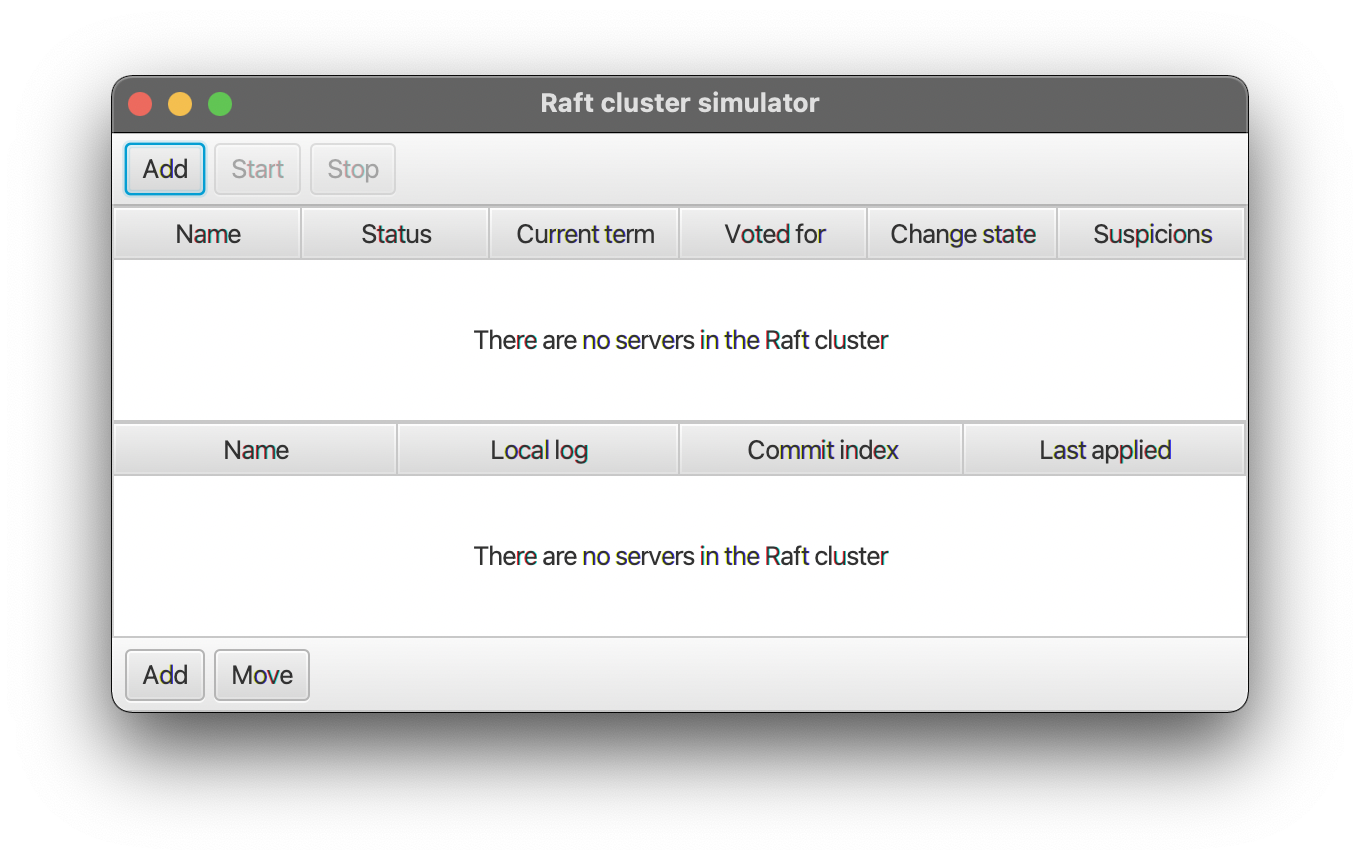
\includegraphics[width=0.66\textwidth]{drawable/init-page.png}
    \caption{The Raft simulator window at start.}
    \label{fig:raft-start}
\end{figure}

The GUI is composed of three sections: the \textit{toolbar}, the \textit{server view}, and the \textit{log view}.

The \textit{toolbar} sits at the top of the window, and is the entrypoint for starting the Raft cluster. It has three buttons, which are dynamically enabled and disabled depending on the context. To get started, press the \textit{Add} button to add a Raft server. Repeat until a satisfactory number of servers is inserted in the system. Note that, once a server has been added, it cannot be removed.

Once at least a server is added to the cluster, the \textit{Start} button is enabled, allowing the system to be started. Since one of the assumptions of the Raft protocol is that the number of servers in the cluster shall not change, once the simulation is started adding more servers is not supported, and the relevant button is grayed out.

In the \textit{server view}, a sortable list of servers is populated as the \textit{Add} button is repeatedly clicked. Fields presented included the name, the status (\texttt{FOLLOWER}/\texttt{CANDIDATE}/\texttt{LEADER}), the current term, and who the server voted in this term. Finally, a button is available on the far right of each right. \autoref{fig:adding-server} shows an example of the GUI once some servers are added.

\begin{figure}[ht]
    \centering
    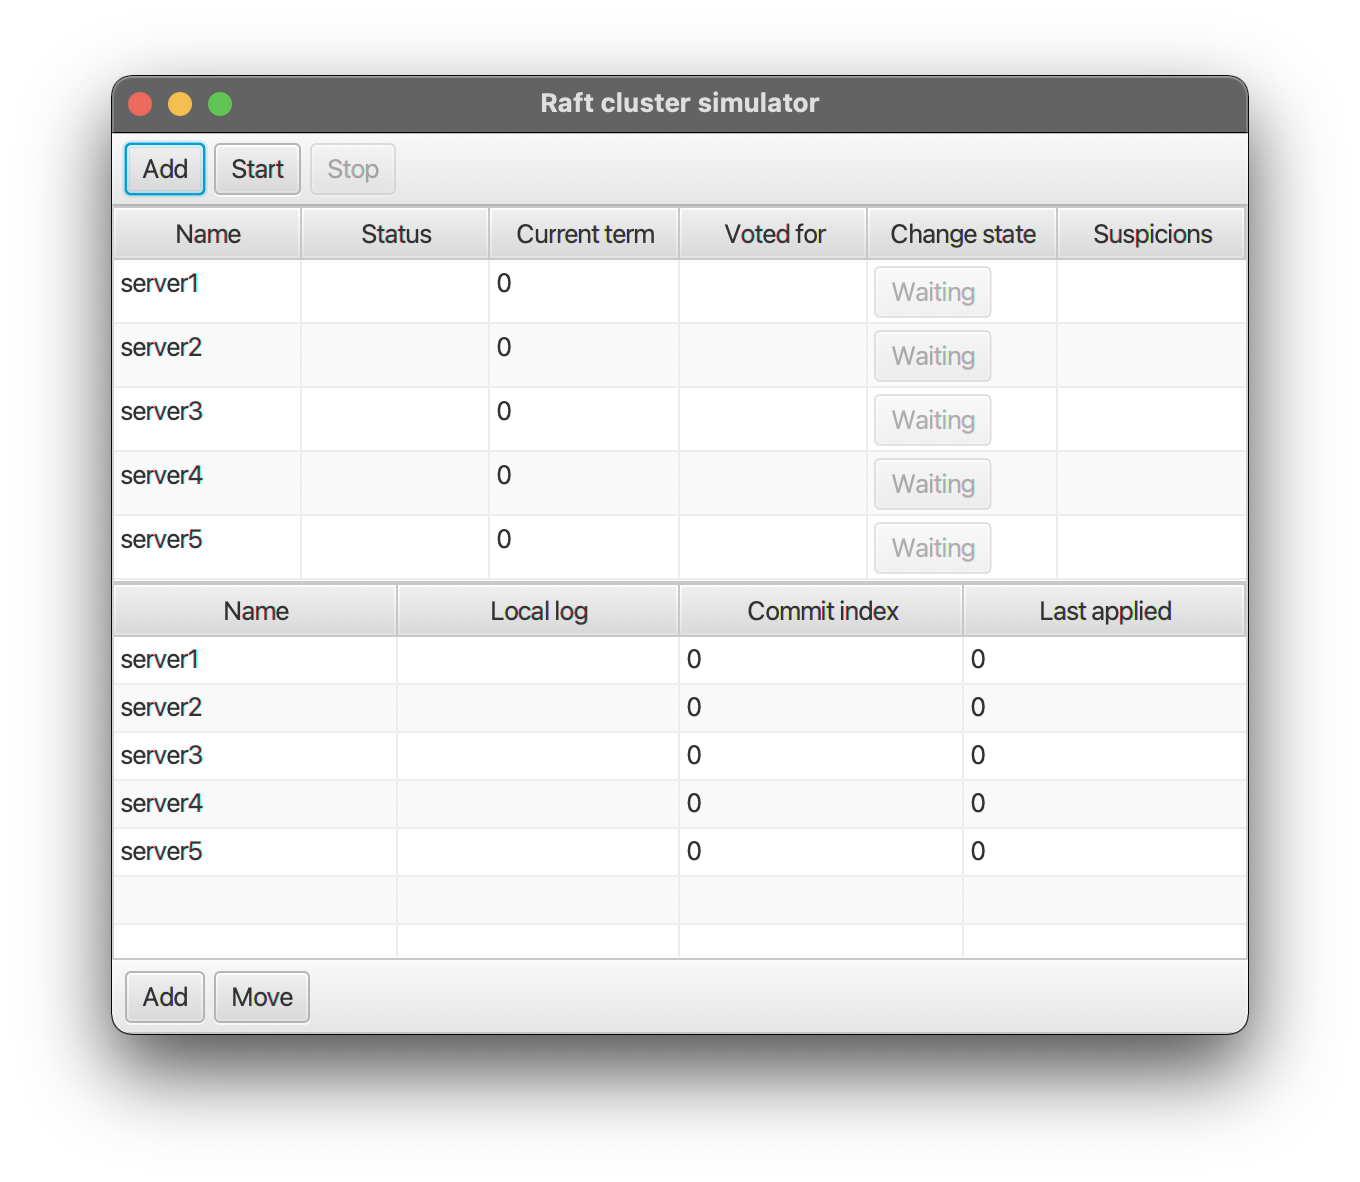
\includegraphics[width=0.66\textwidth]{drawable/adding-few-servers.png}
    \caption{Adding a handful of servers to the simulation.}
    \label{fig:adding-server}
\end{figure}

This button, which is active only when the simulation has been started, allows the user to programmatically crash the related node. The node will stay in a crashed state (i.e. will ignore any incoming message and forget its non-persistent state) until the user presses the button again, effectively rebooting it.

On the bottom \textit{log view}, another table is available which shows the local log, the commit index, and when the commit was last applied. Two additional buttons are available, which allow the user to query the current leader and ask to add an entry to the log.

\subsection{Starting the simulation}

\begin{figure}[ht]
    \centering
    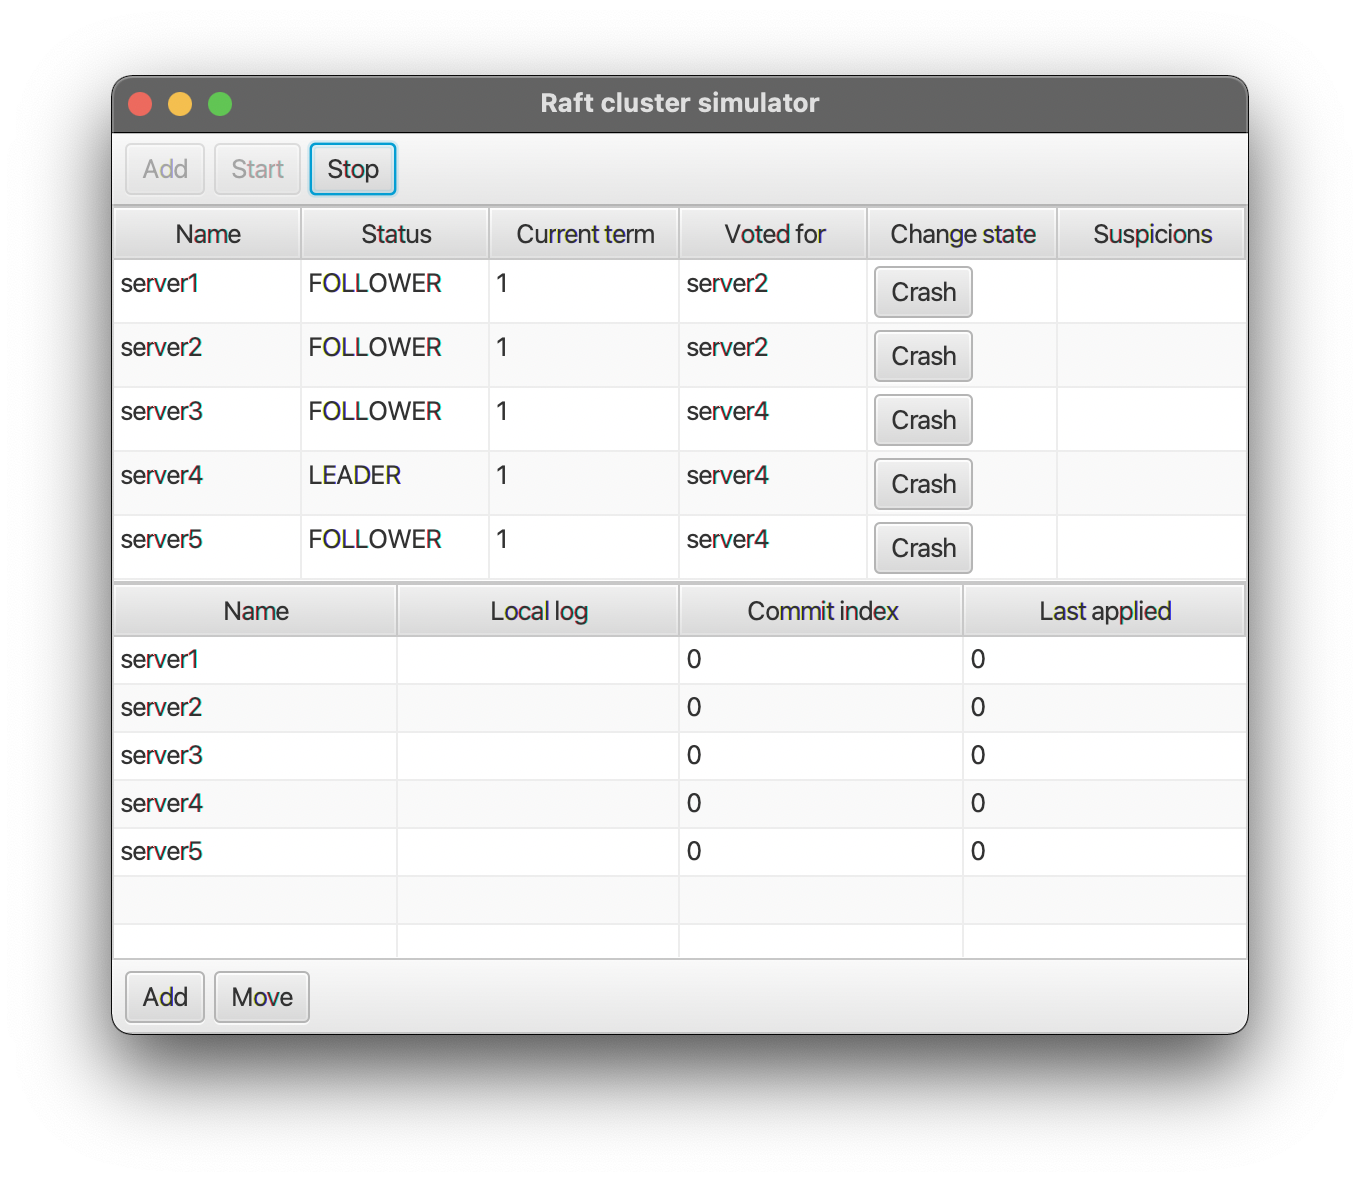
\includegraphics[width=0.44\textwidth]{drawable/1-starting-simulation.png}
    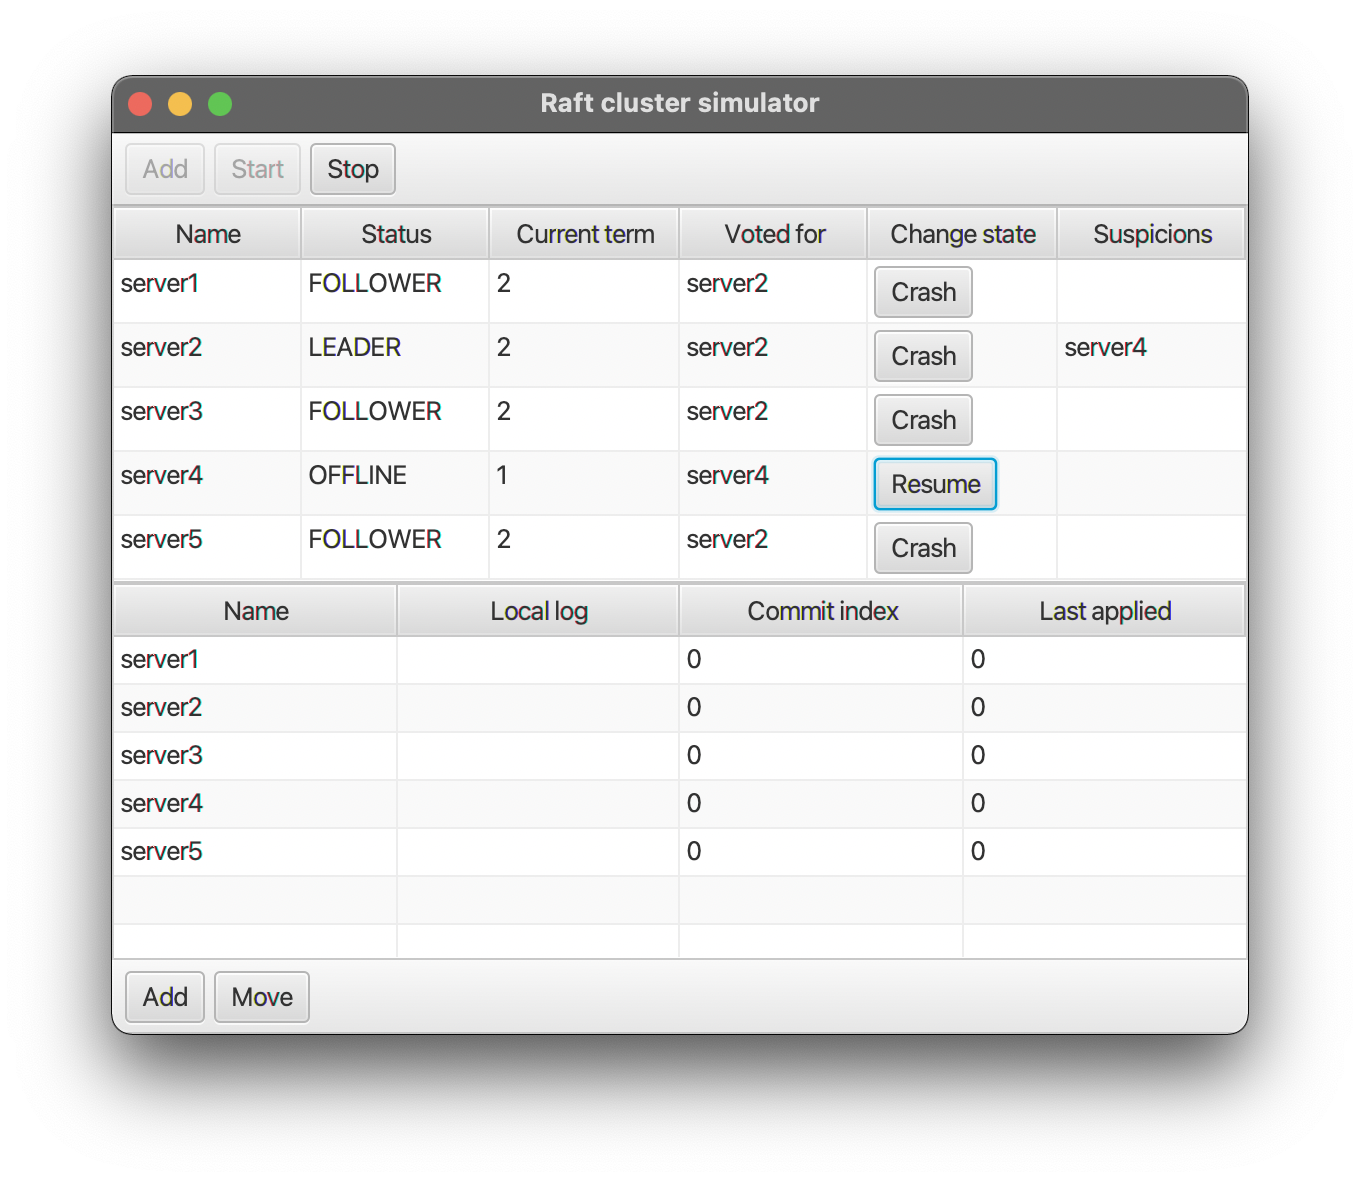
\includegraphics[width=0.44\textwidth]{drawable/2-crashing-leader.png}
    
    \caption{The start of the simulation, and crashing the current leader.}
    \label{fig:starting-simulation-crash}
\end{figure}

Once the user is satisfied with the amount of servers added to the simulation and has started it, the Raft cluster will let every server know each other and let them interact freely using the primitives described in \autoref{architecture}. The servers will set an \texttt{electionTimeout}, and after a short time, one will prevail and will be elected leader. For showcasing purposes, we can crash it with its button. \autoref{fig:starting-simulation-crash} shows an example of what happens in the GUI: as the leader is killed, the other servers' timeouts will expire and will elect a new leader, as they will still be able to meet the majority criteria.


\begin{figure}[ht]
    \centering
    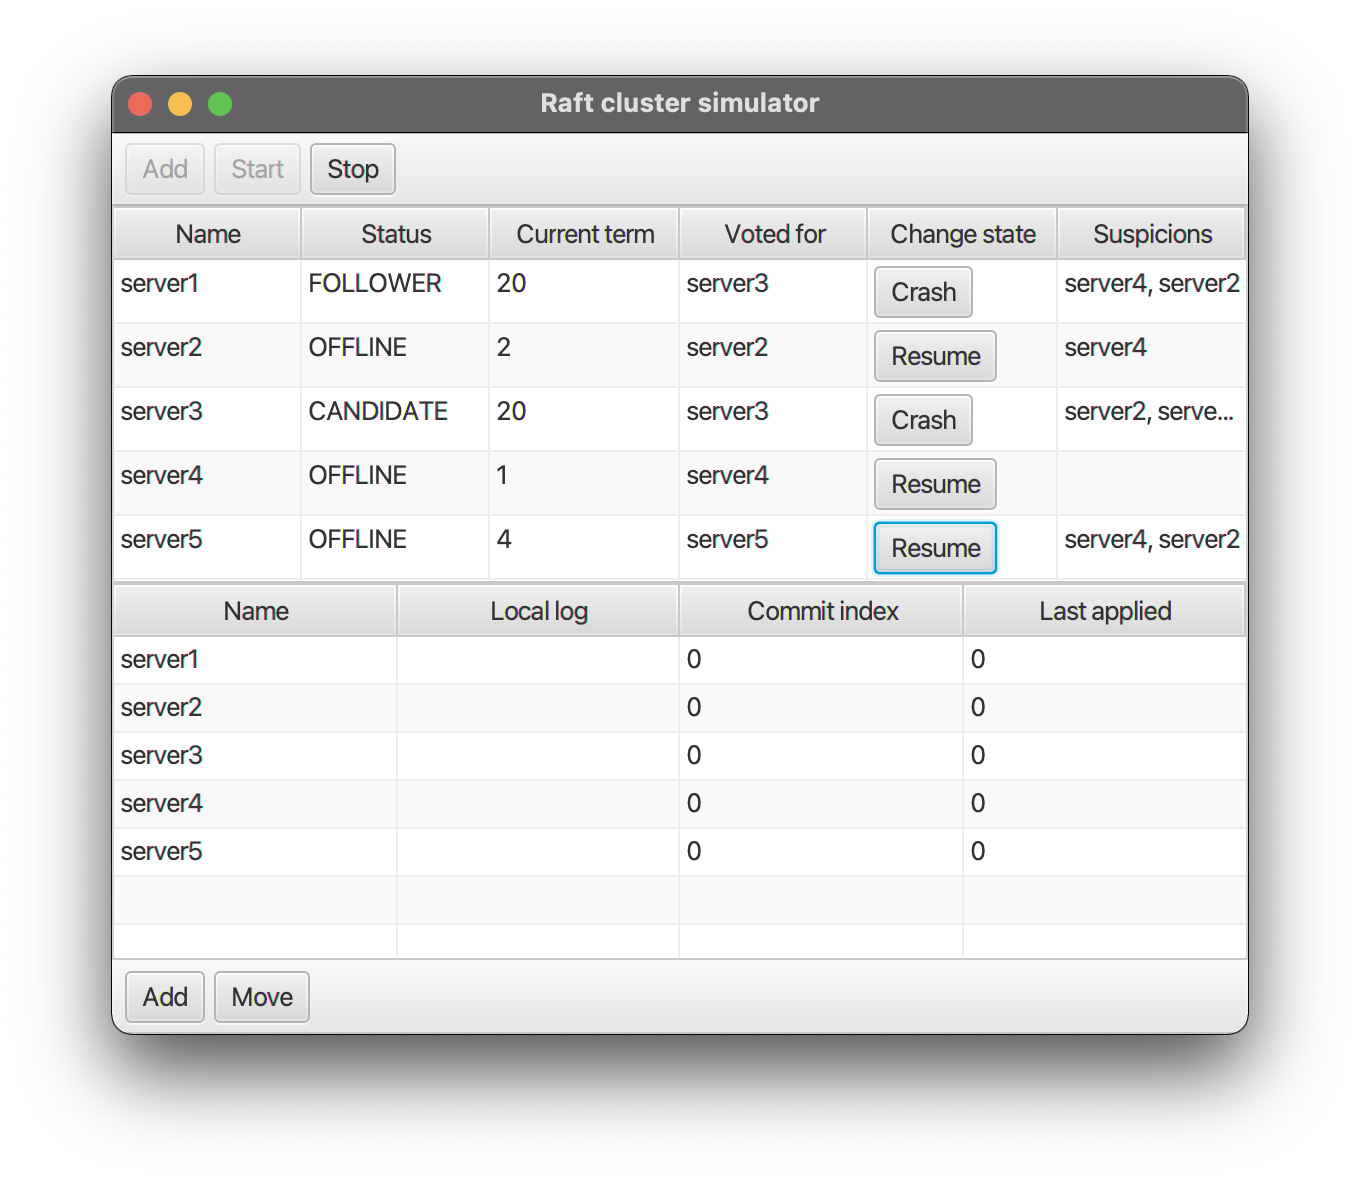
\includegraphics[width=0.44\textwidth]{drawable/2a-chaos-leader.png}
    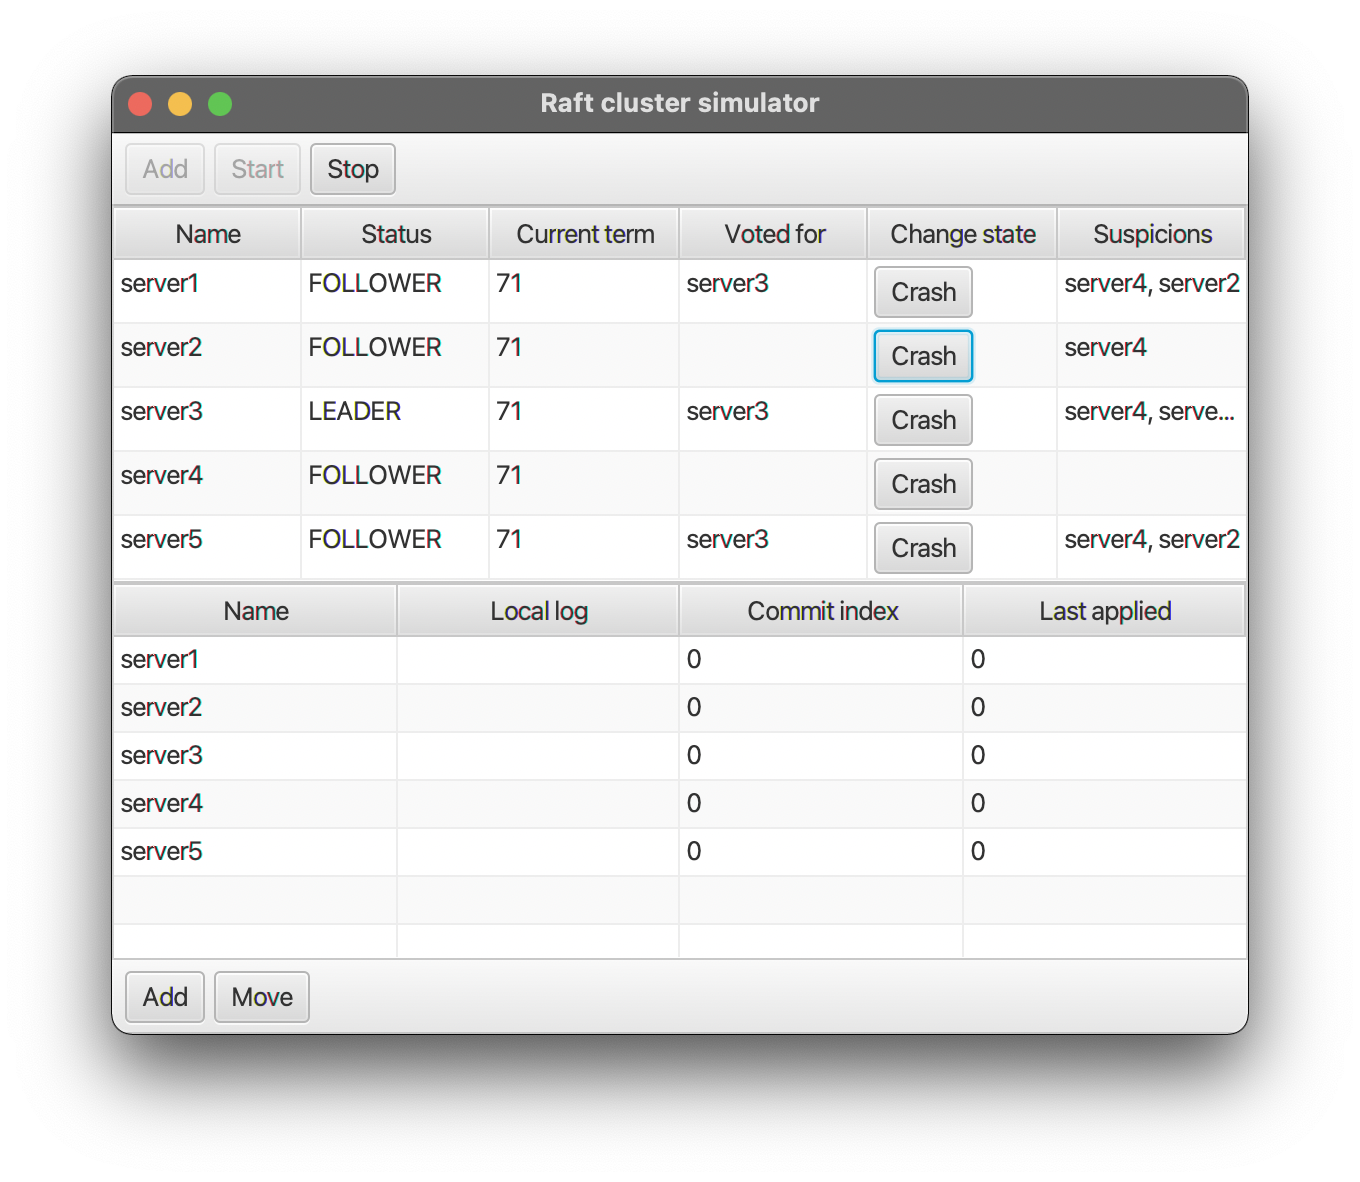
\includegraphics[width=0.44\textwidth]{drawable/3-leader-comeback.png}
    
    \caption{Crashing more than the majority of the servers: to the left, terms start increasing drammatically. To the right, term parity is achieved when they resume from the crash.}
    \label{fig:crash-comeback}
\end{figure}

If the user were to crash more than the majority of the servers, then the remaining servers will start panicking and, as their election timeouts repeatedly expire, start increasing their terms. \autoref{fig:crash-comeback} (left) shows an example of this effect. This is expected behavior, as two servers out of five should never be able to elect a new leader. On the other hand, \autoref{fig:crash-comeback} (right) shows the result of a clean comeback from a crash. The previous leader (\texttt{server2}) came back and was swiftly deposed by the new one, and with the \texttt{appendEntries} messages was informed of the new term and leader. We can observe that \texttt{server2} did not vote for anyone in this term. Again, this is to be expected, as the server was crashed during the election.

\begin{figure}ht
    \centering
    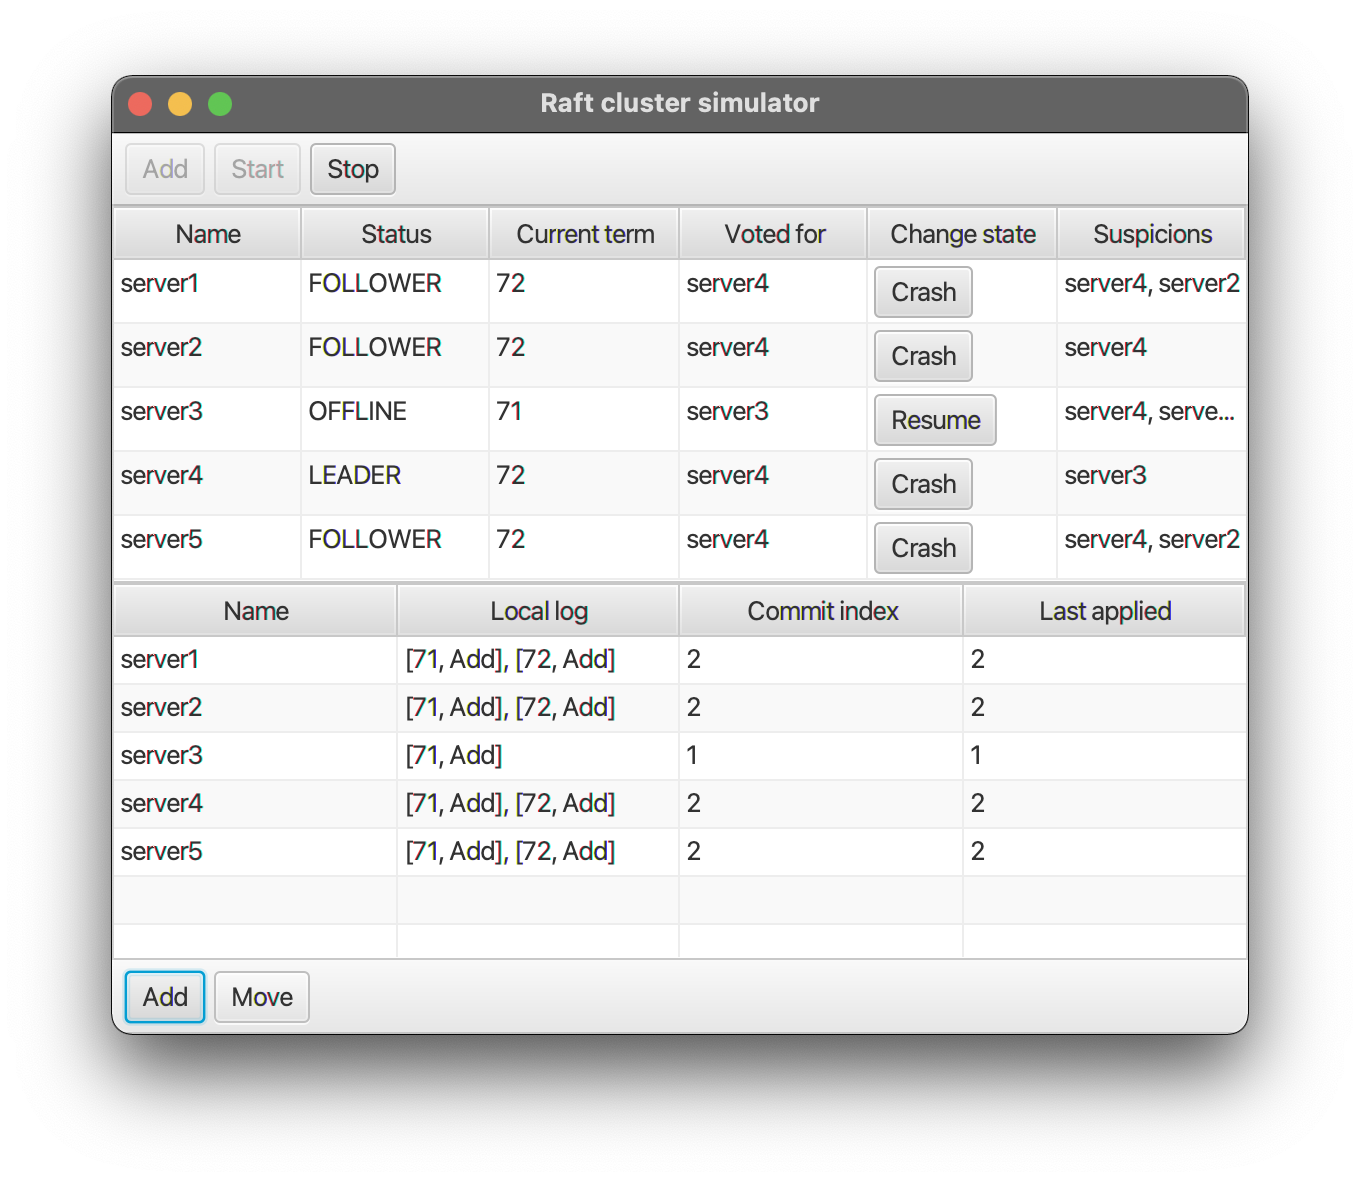
\includegraphics[width=0.66\textwidth]{drawable/4-some-logs.png}
    
    \caption{Adding some logs.}
    \label{fig:adding-logs}
\end{figure}

Finally, \autoref{fig:adding-logs} shows an example of an addition of log entries to the cluster. At first, all servers have recovered from the crashes in previous screenshots. One request is made to the leader of term 71 while all servers are alive. This results in a swift addition to each server's local log. Then, \texttt{server3} is crashed, and an additional request is made to the new leader. Now, every server but \texttt{server3} is aware of the request and has applied it, as the majority was still met even without him. When \texttt{server3} will come back, he will learn with \texttt{appendEntries} messages of the new entries  and will update its local log accordingly.

\subsection{Simulation parameters}

The simulation supports fine tuning of some parameters. This is done via the \verb=simulation.properties= file. The provided file looks like this:

\begin{verbatim}
    timeScale=1
    minElectionTimeoutMs=150
    maxElectionTimeoutMs=800
    heartbeatMs=50
    rpcTimeoutMs=15
    maxCrashDuration=10
\end{verbatim}

The configurable parameters are as following:

\begin{itemize}
    \item \texttt{timeScale}: an integer $\ge 1$. It is used as a factor for other parameters, and allows slowing down the simulation;
    \item \texttt{minElectionTimeoutMs} and \texttt{maxElectionTimeoutMs}: the floor and ceiling values used by the PRNG when computing election timeouts after each \texttt{appendEntries} message;
    %\item \texttt{heartbeatMs}
    \item \texttt{rpcTimeoutMs}: the milliseconds waited by servers before retrying an RPC.
    %\item \texttt{maxCrashDuration}: the maxi
\end{itemize}

\clearpage
\newpage

\input{sections/5\_conclusion.tex}

\clearpage
\newpage

\bibliographystyle{IEEEtran-sorted-tt}
\bibliography{biblio}

\end{document}
